% !TeX encoding = UTF-8
% !TeX program = pdflatex
% !TeX spellcheck = it_IT

\documentclass[binding=0.6cm,TFA]{sapthesis}

\usepackage{microtype}
\usepackage[italian]{babel}
\usepackage[utf8]{inputenc}
\usepackage[hidelinks]{hyperref}
\usepackage{setspace}
\usepackage[Algoritmo]{algorithm}
\usepackage{algorithmic}
\usepackage{graphicx}

\onehalfspacing
\graphicspath{ {assets/} }

\hypersetup{pdftitle={Green IoT: Design e valutazione delle prestazioni di protocolli per sistemi IoT dotati di wake up radio},pdfauthor={Leonardo Emili}}

\title{Green IoT: Design e valutazione delle prestazioni di protocolli per sistemi IoT dotati di wake up radio}
\author{Leonardo Emili}
\IDnumber{1802989}
\course{Informatica L-31}
\courseorganizer{Facoltà di Ingegneria dell'informazione, informatica e statistica}
\AcademicYear{2019/2020}
\copyyear{2020}
\advisor{Prof. Chiara Petrioli}
\tutor{Dr. Georgia Koutsandria}
\tutorcoord{Prof. Chiara Petrioli}
\tutorcoord{Dr. Georgia Koutsandria}
\authoremail{emili.1802989@studenti.uniroma1.it}

\begin{document}
\large

\frontmatter
\maketitle
%\dedication{Dedicato a\\ Donald Knuth}

\tableofcontents

\mainmatter
\chapter{Introduzione}

Nell'ultimo decennio abbiamo assistito ad uno sviluppo portentoso del settore dell'Internet of Things che ha contribuito alla diffusione
di un enorme numero di dispositivi wireless. Il numero di questi dispositivi ha registrato crescite costanti negli anni e loro applicazioni sono ormai infinite.
Essi trovano impiego in ambito domestico dove realizzano l'automatizzazione dei compiti quotidiani, in quello sanitario in cui monitorano lo stato di salute
dei pazienti e in ambito sottomarino dove gli obbiettivi spaziano da quello di realizzare campionamenti di dati sino a creare vaste reti di comunicazione sottomarine.
L'immissione di questo enorme contingente di dati nella rete ha reso possibili nuove interpretazioni e lo sviluppo di soluzioni che puntano a
migliorare la qualità della vita delle persone, anche in quei settori noti esser di difficile comprensione. Ad esempio, l'impiego di sensori IoT in ambito di
monitoraggio del crosta terrestre ha reso disponibili informazioni fino a prima sconosciute sulla presenza di terremoti e tsunami, migliorando radicalmente
la nostra percezione degli eventi sismici nel mondo.\\

Con lo sviluppo massivo dell'IoT nuove sfide sono emerse a minare la solidità degli approcci usati. Attualmente le soluzioni impiegate nello sviluppo
dei dispositivi wireless puntano a realizzare comunicazioni con basse latenze e che siano altamente efficienti in termini energetici. In ambito di ricerca,
lo stato corrente dell'arte punta a realizzare tecnologie hardware e software che implementino questo binomio. Un particolare
settore dell'IoT si occupa di realizzare vaste reti di nodi sensori interconnessi, note come \emph{Wireless Sensor Networks},
che realizzano una comunicazione wireless con consumi minimi al fine di prolungare i tempi di servizio dell'intera rete. In questo caso,
le principali problematiche sono chiaramente settoriali e sono identificate dallo specifico campo di applicazione: come la richiesta di tecnologie
altamente performanti per i monitoraggio clinici oppure di altre che garantiscano elevate lifetime nel caso di sensori ambientali. Tuttavia esistono
problematiche comuni a queste tipologie di reti, ad esempio spesso si richiede che l'intera rete sia connessa e che tutti i nodi siano,
anche parzialmente, a conoscenza della topologia della rete. Nel caso, si richiede l'impiego di protocolli che ne prevedano il
costante aggiornamento e favoriscano una comunicazione efficiente. Inoltre, in queste reti la principale fonte di consumo energetico risiede
nella comunicazione e nell'attesa che la precede, è quindi di vitale importanza prevedere che i nodi della rete siano
oggetto di scaricamento delle batterie che li alimentano. Infatti, la morte prematura di un nodo può spesso avere conseguenze più grandi della semplice
disconnessione dello stesso, poichè frequentemente si tratta di reti \emph{multi-hop} che realizzano la comunicazione passando attraverso nodi intermedi, si può
verificare perfino la disconnessione dell'intera rete.\\

Nel seguito verranno descritte le principali problematiche che motivano ricerca di nuove idee per la costruzione di protocolli di rete efficienti.
Nel capitolo seguente analizzeremo lo scenario di riferimento e le principali considerazioni che nel tempo sono state adottate e che ad oggi
definiscono il panorama delle Wireless Sensor Networks.\\

Nel capitolo 3 verrà presentato uno specifico protocollo di rete per sistemi IoT: il protocollo GREEN-WUP. In questo lavoro ci concentreremo sullo
studio dei principi che regolano il design dei protocolli di rete e sulla loro applicazione in riferimento al protocollo in questione. Analizzeremo
in dettaglio il comportamento del protocollo, descrivendone i principali vantaggi e le problematiche.\\

Nel capitolo 4 verrà presentata una variante del protocollo originale che punta a risolvere le problematiche osservate nel capitolo precedente. Le
modifiche apportate saranno descritte in dettaglio sia a livello teorico che a livello di implementazione all'interno di Castalia,
simulatore utilizzato a cui faremo diffusamente riferimento all'interno di questa relazione.\\

Nel capitolo 5 saranno analizzate le prestazioni della variante proposta e quelle del protocollo originale. In particolare, verranno mostrati i
comportamenti di entrambe le implementazioni all'interno di uno stesso ambiente reale ed infine nel Capitolo 6 trarremo le conclusioni di quanto osservato.


\chapter{Scenario di riferimento}

Sino a qualche anno fa, la principale tendenza nello sviluppo di soluzioni ai problemi menzionati nel Capitolo 1 consisteva nell'introduzione di cicli di attività
dei nodi. Il cosiddetto \emph{duty cycling}, definito come la frazione di tempo in cui un nodo è attivo, aveva come obbettivo quello di minimizzare i momenti
in cui i nodi sensori sono accessi senza alcun processamento di dati attivo. Seppur questo approccio permetta di prolungare la durata della vita della rete,
incrementa in maniera considerevole i ritardi nelle comunicazioni, dal momento che queste possono avvenire solamente all'interno delle finestre di attività
delle coppie dei nodi coinvolti. Tuttavia l'utilizzo del duty cycling non permette di risolvere tutti i problemi in quanto le comunicazioni possono ancora
avvenire nei momenti di inattivà dei nodi. Dualmente, esistono ancora i periodi di tempo in cui i nodi consumano energia pur non ricevendo o inviando dati.\\


In questo panorama vengono introdotte le \emph{wake up radios}, in grado di abbattere i consumi energetici mantenendo bassi i ritardi nelle comunicazioni.
La principale differenza rispetto all'approccio tradizionale consiste nell'introdurre un'antenna secondaria per i soli messaggi di wake-up costantemente
attiva. La nuova antenna è progettata per avere di dimensioni ridotte e consumi energetici nettamente inferiori rispetto a quelli della radio principale.
Al momento della ricezione di un messaggio di wake-up è possibile attivarla e ricevere il pacchetto dati. Di fatto questa tecnologia implementa uno schema
di comunicazione \emph{on demand}: un nodo può inviare un pacchetto dati ad un nodo dormiente semplicemente  posticipandone l'invio a quello di una sequenza
di wake-up che, svegliando il ricevente, lo abilita alla ricezione. In questo modo i nodi possono rimanere attivi per il solo tempo minimo necessario a
svolgere l'attività richiesta e lasciare spenta la radio principale nel tempo rimanente. Dal punto vista energetico questo approccio è altamente efficiente
e non richiede alcuna forma di sincronizzazione che è generalmente non desiderata in quanto implicitamente introduce overhead dovuto alla gestione di timer
aggiuntivi.\\

Più recentemente la tendenza è quella di equipaggiare i nodi sensori, dotati di wake up radios, con moduli per l'\emph{energy harvesting} come ulteriore
supporto energetico alla loro durata di attività. In particolare, i nodi sono in grado di utilizzare l'energia fornita dalle pile elettriche di cui sono
forniti e di derivarne nuova mediante turbine eoliche, pannelli solari e generatori termoelettrici di cui sono equipaggiati. La ricerca ha dimostrato che
l'impiego di nodi dotati di energy harvesting \cite{energy-harvesting-paper} e che sono abilitati alle wake up radios \cite{wake-up-radios-paper} ha
portato notevoli incrementi nelle performance delle Wireless Sensor Networks.\\

Inoltre, l'innovativa tecnologia delle wake up radios può essere combinata con il cosiddetto \emph{semantic addressing}. L'idea in questo caso è di limitare
ad un sottoinsieme di nodi la ricezione di una sequenza di wake up, evitando quindi che questa sia recepita da tutti i nodi presenti all'interno
del range di comunicazione. Il principio fondante è quello di scegliere una o più opportune sequenze di wake up e di assegnarle ad un certo
sottoinsieme di nodi della rete. A meno di errori di interpretazione della sequenza di wake up, al momento della ricezione tutti e soli e nodi desiderati
saranno svegliati. In questo scenario, i consumi energetici risultano essere ulteriormente ridotti poichè viene virtualmente azzerato il numero dei nodi
che sono riattivati a seguito di sequenze di wake up non a loro destinate ma che si trovano all'interno del loro range.\\

Questo lavoro si concentra sullo studio di protocolli delle cosiddette \emph{green wireless sensor network}, ovverosia di quei protocolli che si basano
sulle tecnologie sopra esposte e che implementano la comunicazione tra nodi minimizzandone gli sprechi energetici al fine di massimizzare
i tempi di attività e il corretto funzionamento delle comunicazioni all'interno delle reti. Nella letteratura scientifica
sono presenti molti protocolli di questo tipo (es. CTP-WUR, GREENROUTES, WHARP) e ciascuno di loro punta a risolvere diverse problematiche.
Nel seguito verrà analizzato in dettaglio il comportamento del protocollo GREEN-WUP che utilizza energy harvesting e wake up radio per realizzare
un'opportuna scelta del percorso da seguire per permettere la ricezione dati da parte del sink node.\\

\chapter{Il protocollo GREEN-WUP}

Il protocollo GREEN-WUP si inserisce nel contesto dei protocolli delle \emph{green wireless sensor network} e pone tra i suoi principali obiettivi
la massima efficienza energetica della rete. Esso impiega le tecnologie di wake up radio, energy harvesting e semantic addressing. Inoltre, è
di tipo \emph{converge casting} ed è basato sull'assegnazione di hop count a ciascun nodo per poter distribuire i pacchetti dati
all'interno della rete.\\

L'approccio tradizionale dei protocolli di rete prevede due fasi principali: in primo luogo avviene la fase di \emph{interest dissemination} dove si
definisce la topologia della rete da rispettare affinchè i nodi realizzino un corretto flusso di scambio dati; successivamente si assume che gli
indirizzi di wake up siano stati assegnati e si procede con lo scambio di dati che è governato da sequenze di wake up che vengono utilizzate per
risvegliare i nodi della rete. Nel caso specifico di GREEN-WUP la fase di interest dissemination non viene eseguita per motivi di efficienza
e gli hop count vengono determinati indirettamente prima ancora dell'inizio della simulazione. Per ragioni completezza in questo lavoro verrà
mostrata sia alla versione originale di GREEN-WUP che non comprende la fase di interest dissemination che una versione che la utilizza per
il calcolo degli hop count dei nodi della rete.\\

In GREEN-WUP ciascun nodo è fornito di una coppia di indirizzi di wake up. Si tratta infatti di un primo indirizzo che identifica univocamente
il nodo nella rete e rimane invariato nel tempo e di un altro che è mutabile nel tempo ed è definito a partire dallo stato corrente del nodo.
Quest'ultimo indirizzo di wake up è definito da una sequenza $w=w_{h}w_{e}$ della lunghezza di 8 bit, dove $w_{h}$ rappresenta il valore di hop
count $h$ del nodo in questione, $w_{e}$ invece rappresenta la sua attuale classe energetica. Si noti come questo secondo indirizzo di venga
aggiornato periodicamente per riflettere la sua disponibilità energetica nel tempo. Questa idea realizza il principio del semantic addressing
poiché in questo scenario è possibile far riferimento ad un sottoinsieme di nodi della rete a partire dai loro valori di hop count
e da quello della classe energetica. \\

%image source: https://www.researchgate.net/figure/Topology-of-wireless-sensor-network-and-hop-count-of-sensors_fig7_285956270
\begin{figure}
    \begin{center}
        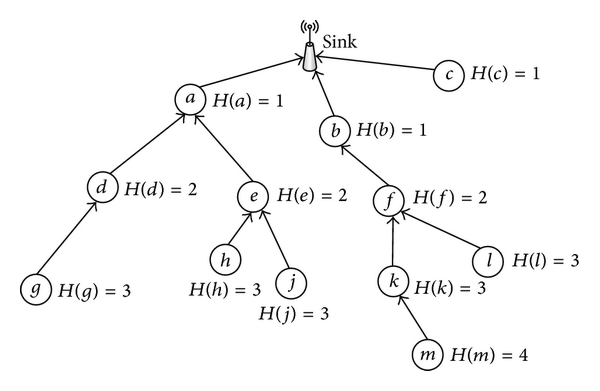
\includegraphics[scale=1.7]{hop-count-algorithm.png}
        \caption{Topologia della rete a seguito dell'assegnazione degli hop count.}
    \end{center}
\end{figure}

Nel momento in cui un nodo deve inviare un pacchetto dati può farlo seguendo degli step fondamentali di seguito descritti.
La prima fase consiste nell'instaurare una comunicazione con i nodi elegibili alla ritrasmissione del pacchetto: il suddetto nodo sensore
entra in uno stato di ricerca di un nodo che si farà carico della sua richiesta di ritrasmissione. La ricerca si considera conclusa
nel momento in cui viene selezionato un nodo tra quelli disponibili come nodo intermediario tra il nodo che invia i dati (sender) e il sink
node, cui la richiesta di ricezione dati è destinata. Infine si procede alla trasmissione del pacchetto, a seguito della quale
verrà inviata una conferma a certificare l'avvenuta ricezione dello stesso e si ripete in questo modo sino a raggiungere
il sink node.\\

Nel seguito sarà descritto il comportamento del protocollo da un punto di vista algoritmico ed in seguito alcune osservazioni su di esso.
Per facilitarne la lettura, il duplice ruolo che ciascun nodo assume viene scomposto in due parti: rispettivamente in \textbf{Algoritmo 1}
viene descritto il comportamento che ciascun nodo assume nel momento in cui deve inviare dei dati (sender), mentre in \textbf{Algoritmo 2}
viene descritto il comportamento che questo assume quando agisce da nodo intermediario (receiver).

\begin{algorithm}
    \caption{Sender in GREEN-WUP}
    \begin{algorithmic}
        \REQUIRE $level > 0$

        \WHILE{queue is not empty}
            \STATE $dataPkt \leftarrow$ queue.head()
            %\STATE do CSMA/CA and backoff until channel is CLEAR

            \IF{level = 1}
                \STATE send $dataPkt$ to the sink node and wait for some time $\delta_{ACK}$ to receive the relative ACK packet

            \ELSE
                \STATE $k \leftarrow$ maxEnergyClass
                \STATE $acked \leftarrow$ false
                \WHILE{$k>0$ $and$ not $acked$}
                    \STATE $address_{RTS} \leftarrow$ createWurAddress(level - 1, k)
                    \STATE send $address_{RTS}$ and wait for nearby nodes to wake up
                    \STATE $rtsPkt \leftarrow$ createRTS(self)
                    \STATE send $rtsPkt$ in broadcast and wait for some time $\delta_{CTS}$
                    
                    \IF{CTS packet is received within $\delta_{CTS}$}
                        \STATE send a wake up signal using the address contained inside the first CTS packet received and wait for the receiver to wake up
                        \STATE send $dataPkt$ and wait for some time $delta_{ACK}$

                        \IF{ACK packet is received within $\delta_{ACK}$}
                            \STATE $acked \leftarrow$ true
                        \ENDIF
                    \ENDIF
                    \STATE $k \leftarrow k-1$
                \ENDWHILE
            \ENDIF
        
        \ENDWHILE
    \end{algorithmic}
\end{algorithm}

\begin{algorithm}
    \caption{Receiver in GREEN-WUP}
    \begin{algorithmic}
        \REQUIRE the node detects a wake up signal $address_{RTS}$

            \STATE activate the main radio and wait for some time $\delta_{RTS}$

            \IF{RTS packet is received within $\delta_{RTS}$}
                \STATE $\delta_{JITTER} \leftarrow$ random value in $[0,maxJitter)$
                \STATE wait for $\delta_{JITTER}$ and then send a wake up signal using the address contained inside the RTS packet
                \STATE $ctsPkt \leftarrow$ createCTS(self)
                \STATE send $ctsPkt$ and wait for some time $\delta_{DATA}$

                \IF{DATA packet is received within $\delta_{DATA}$}
                    \STATE send an acknowledgement packet to the sender
                \ENDIF
            \ENDIF

            \STATE process buffered packets if there are any, otherwise go back to sleep
        
    \end{algorithmic}
\end{algorithm}

Si noti come in \textbf{Algoritmo 1} si abbia come precondizione fondamentale che il valore di hop count (\emph{level}) sia maggiore strettamente
di zero in quanto il design del protocollo preveda che il sink node agisca da mero destinatario delle comunicazioni della rete. Si osservi come
nel caso in cui il nodo sia a diretto contatto con il sink node ($level=1$) la trasmissione del pacchetto dati avvenga senza alcuna forma di
selezione del nodo intermedio, in quanto superflua. D'altra parte se il nodo non può trasmettere direttamente il pacchetto al sink node ($level>1$)
si procede contattando i nodi vicini al nodo in questione. I nodi candidati vengono considerati in base alla loro classe energetica corrente,
a partire dai nodi con classe energetica massima \\

La descrizione teorica del protocollo non comprende le fasi di CSMA/CA and backoff until channel is CLEAR e di retries che vengono fatti
per l'invio di ciascun pacchetto in quanto sono comuni a tutti i protocolli di rete.

\chapter{Soluzioni proposte}

\begin{algorithm}
    \caption{Sender nella variante}
    \begin{algorithmic}
        \REQUIRE $level > 0$

        \WHILE{queue is not empty}
            \STATE $dataPkt \leftarrow$ queue.head()

            \IF{level = 1}
                \STATE send $dataPkt$ to the sink node and wait for some time $\delta_{ACK}$ to receive the relative ACK packet

            \ELSE
                \STATE $k \leftarrow$ maxEnergyClass
                \STATE $acked \leftarrow$ false
                \WHILE{$k>0$ $and$ not $acked$}
                    \STATE $u \leftarrow$ maxBufferClass
                    \WHILE{$u>0$ $and$ not $acked$}
                        \STATE $address_{RTS} \leftarrow$ createWurAddress(level - 1, k, u)
                        \STATE send $address_{RTS}$ and wait for nearby nodes to wake up
                        \STATE $rtsPkt \leftarrow$ createRTS(self)
                        \STATE send $rtsPkt$ in broadcast and wait for some time $\delta_{CTS}$
                        
                        \IF{CTS packet is received within $\delta_{CTS}$}
                            \STATE send a wake up signal using the address contained inside the first CTS packet received and wait for the receiver to wake up
                            \STATE send $dataPkt$ and wait for some time $delta_{ACK}$

                            \IF{ACK packet is received within $\delta_{ACK}$}
                                \STATE $acked \leftarrow$ true
                            \ENDIF
                        \ENDIF
                        \STATE $u \leftarrow u-1$
                    \ENDWHILE
                    \STATE $k \leftarrow k-1$
                \ENDWHILE
            \ENDIF
        
        \ENDWHILE
    \end{algorithmic}
\end{algorithm}

\begin{algorithm}
    \caption{Receiver nella variante}
    \begin{algorithmic}
        \REQUIRE $s+p=1$, the node detects a wake up signal $address_{RTS}$

            \STATE $r \leftarrow$ random value in $[0,maxEnergy]$
            \IF{$r < predictEnergy($t$)$}
                \STATE activate the main radio and wait for some time $\delta_{RTS}$

                \IF{RTS packet is received within $\delta_{RTS}$}

                    \STATE $\delta_{W} \leftarrow$ random value in $[0,maxJitter)$
                    \STATE $\delta_{E} \leftarrow$ $(maxJitter-\delta_{W}) \cdot s \cdot (1 - energyRatio)$
                    \STATE $\delta_{B} \leftarrow$ $(maxJitter-\delta_{W}) \cdot p \cdot bufferState$
                    \STATE $\delta_{JITTER} \leftarrow$ $\delta_{W} + \delta_{E} + \delta_{B}$
                    \STATE wait for $\delta_{JITTER}$ and then send a wake up signal using the address contained inside the RTS packet
                    \STATE $ctsPkt \leftarrow$ createCTS(self)
                    \STATE send $ctsPkt$ and wait for some time $\delta_{DATA}$

                    \IF{DATA packet is received within $\delta_{DATA}$}
                        \STATE send an acknowledgement packet to the sender
                    \ENDIF
                \ENDIF

                \STATE process buffered packets if there are any, otherwise go back to sleep
            \ENDIF
        
    \end{algorithmic}
\end{algorithm}

\chapter{Valutazione delle prestazioni}
\chapter{Conclusioni}

\backmatter
\cleardoublepage
\phantomsection % Give this command only if hyperref is loaded
\addcontentsline{toc}{chapter}{\bibname}

\begin{thebibliography}{9}

    \bibitem{energy-harvesting-paper}
    Stefano Basagni, Georgia Koutsandria, Chiara Petrioli.
    \textit{A Comparative Performance Evaluation of Wake-up Radio-based Data Forwarding for Green Wireless Networks}.

    \bibitem{wake-up-radios-paper}
    Stefano Basagni, Valerio Di Valerio, Georgia Koutsandria, Chiara Petrioli.
    \textit{Wake-up Radio-enabled Routing for Green Wireless Sensor Networks}
\end{thebibliography}

\end{document}